% For Appendix A if needed

\chapter{Supporting Topics}

\section{Sub-Portfolio Selection Based on $p_{\cap}$}
Based on the discussion in Chapter Four, the optimal values of $p_{\cap}$ for IPC2018, MAXSAT19-UCMS, SAT11-INDU, SAT18-EXP, and SAT16-MAIN are 0.59, 0.55, 0.63, 0.81, and 0.33, respectively for regression random-forest performance model. In the following, some examples of the prediction distribution curves are plotted per scenario.
Figure~\ref{fig:appendix_ipc2018} shows two instances from the IPC2018 scenario, \textit{nurikabe\_p03.pddl} (left) and \textit{caldera\_p03.pddl} (right). Since the optimal value of $p_{\cap}$ for this scenario is 0.59, for each instance we choose the solvers whose overlap area with the minimum predicted solver is greater than 0.59. Based on this method, for \textit{nurikabe\_p03.pddl}, \textit{blind}, \textit{Delfi1}, \textit{FDMS2}, \textit{symbolic.bidirectional}, and \textit{DecStar} will be chosen to run in parallel, while \textit{blind} is the VBS and also the best predicted solver. For the \textit{caldera\_p03.pddl} instance, two solvers are selected: \textit{Metis1} and \textit{Metis2}. In this instance, the Virtual Best Solver (VBS) is also the blind solver, but the solver with the minimum predicted time is \textit{Metis1}.

The same situation exists with the MAXSAT19-UCMS scenario, where the optimal $p_{\cap}$ is 0.55. Figure~\ref{fig:appendix_maxsat} shows that based on the optimal $p_{\cap}$ for the \textit{wolfram72\_9.wcnf} instance (left), the \textit{UWrMaxSat.1.0}, \textit{maxino2018} and \textit{MaxHS} solvers should be selected. For this instance, \textit{UWrMaxSat.1.0} is the best predicted solver, and \textit{MaxHS}, which is included in the portfolio, is the actual best solver. For the \textit{1bpi\_2knt\_gwcnft.wcnf} instance (right), all solvers except \textit{MaxHS} are selected in the portfolio, and the VBS (Virtual Best Solver) \textit{QMaxSAT2018} is included in the subportfolio. The same situation exists with the SAT scenarios; however, due to the large number of solvers in those scenarios, the plots are omitted here.

\begin{figure}
    \centering 
    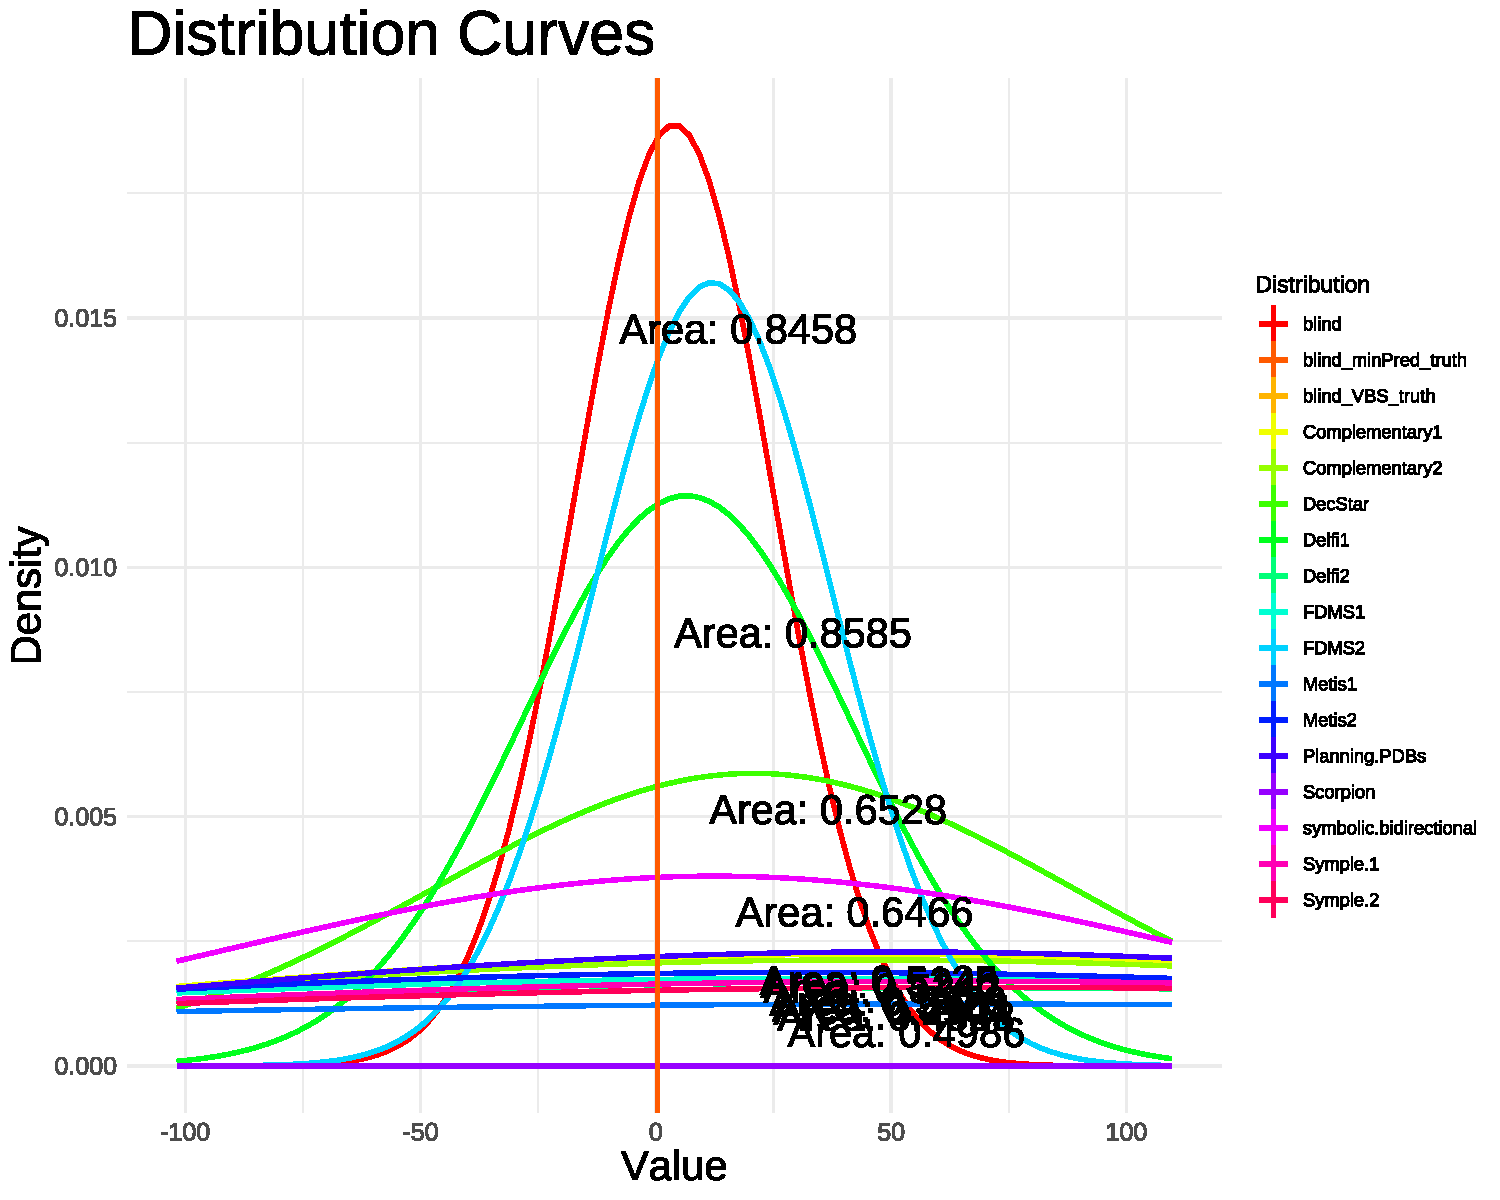
\includegraphics[width=.49\textwidth]{plots/Appendix/nurikabe_p03.pddl.pdf}
    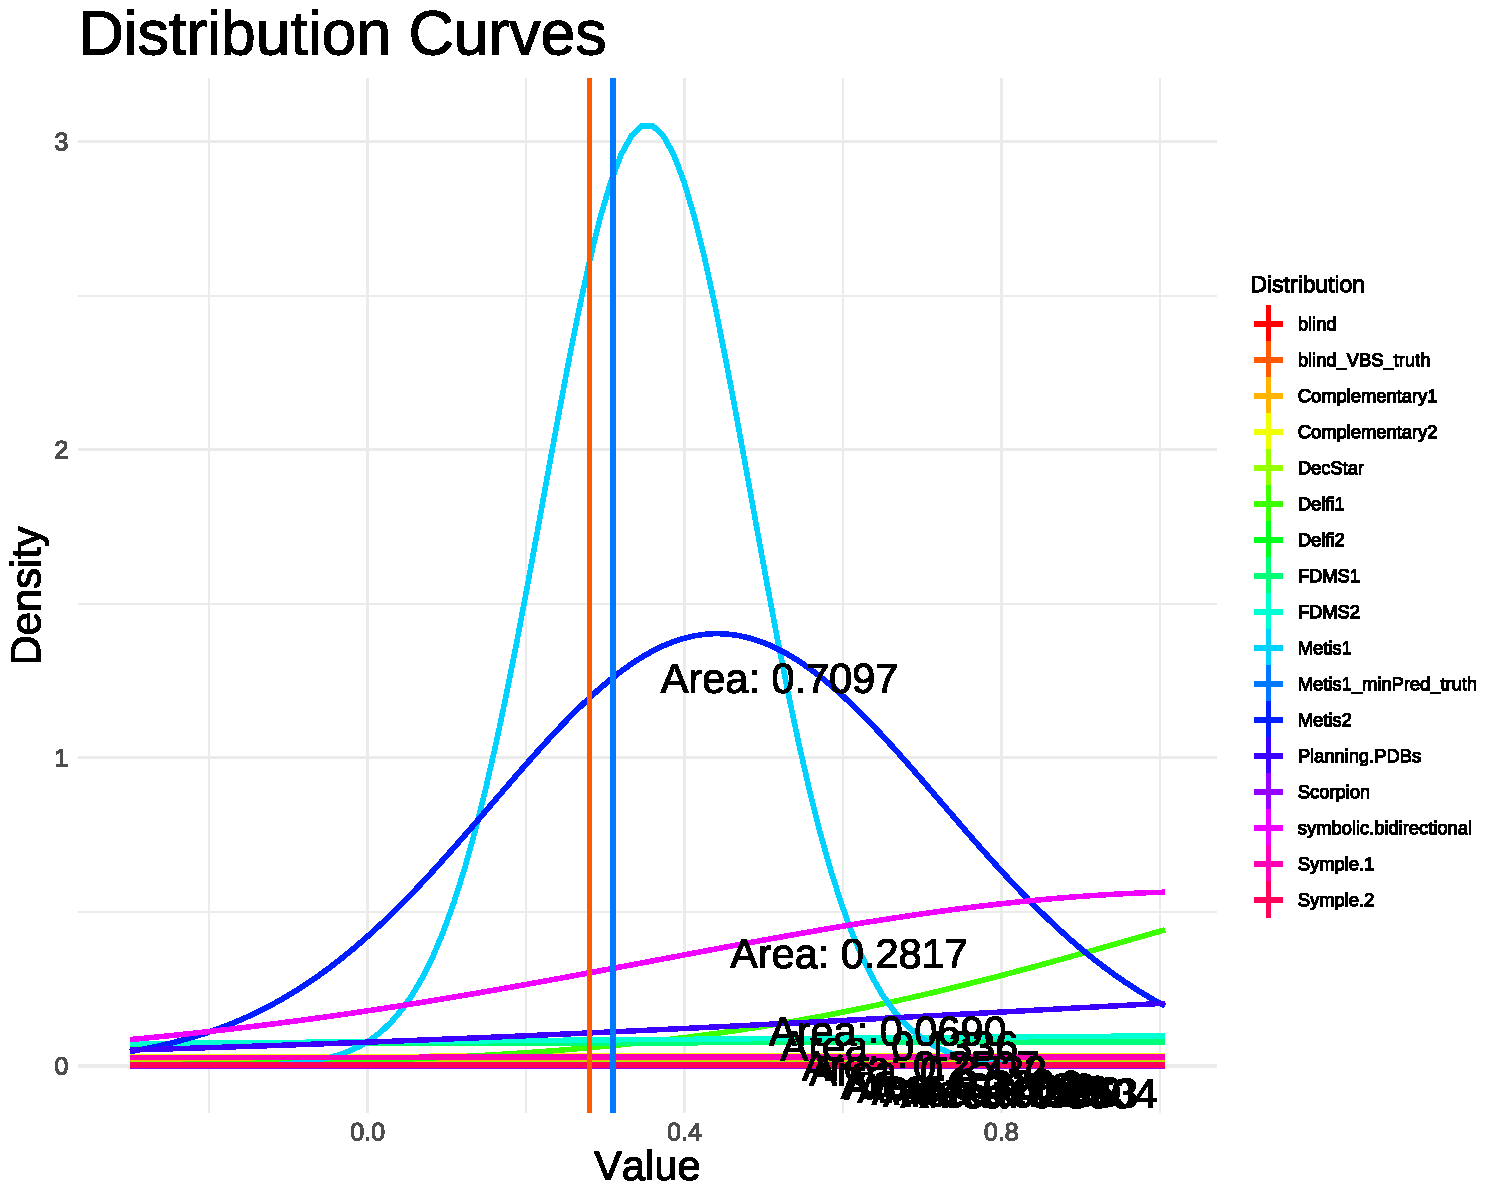
\includegraphics[width=.49\textwidth]{plots/Appendix/caldera_p03.pddl.pdf}
    \caption[Sub-portfolio Selection: Examples from IPC2018]{Sub-portfolio selection for two example instances from IPC2018 based on the optimal $p_{\cap}$ values}
    \label{fig:appendix_ipc2018}
\end{figure}
\begin{figure}
    \centering 
    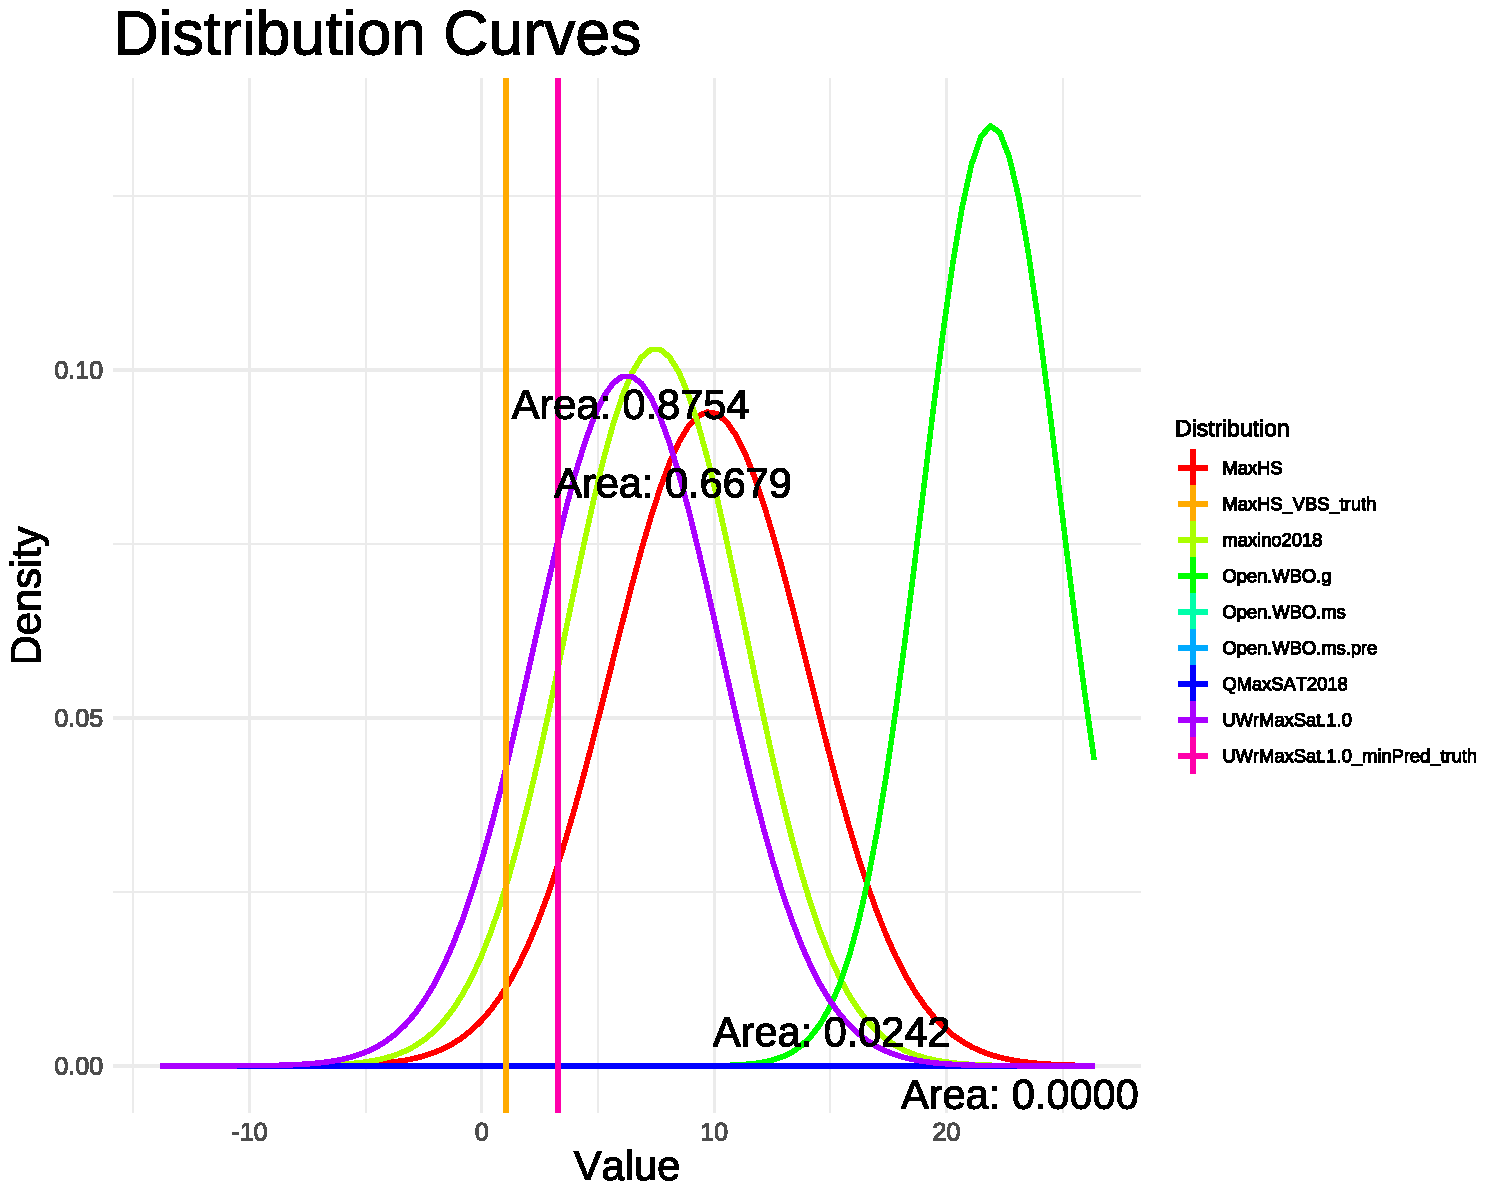
\includegraphics[width=.49\textwidth]{plots/Appendix/wolfram72_9.wcnf.pdf}
    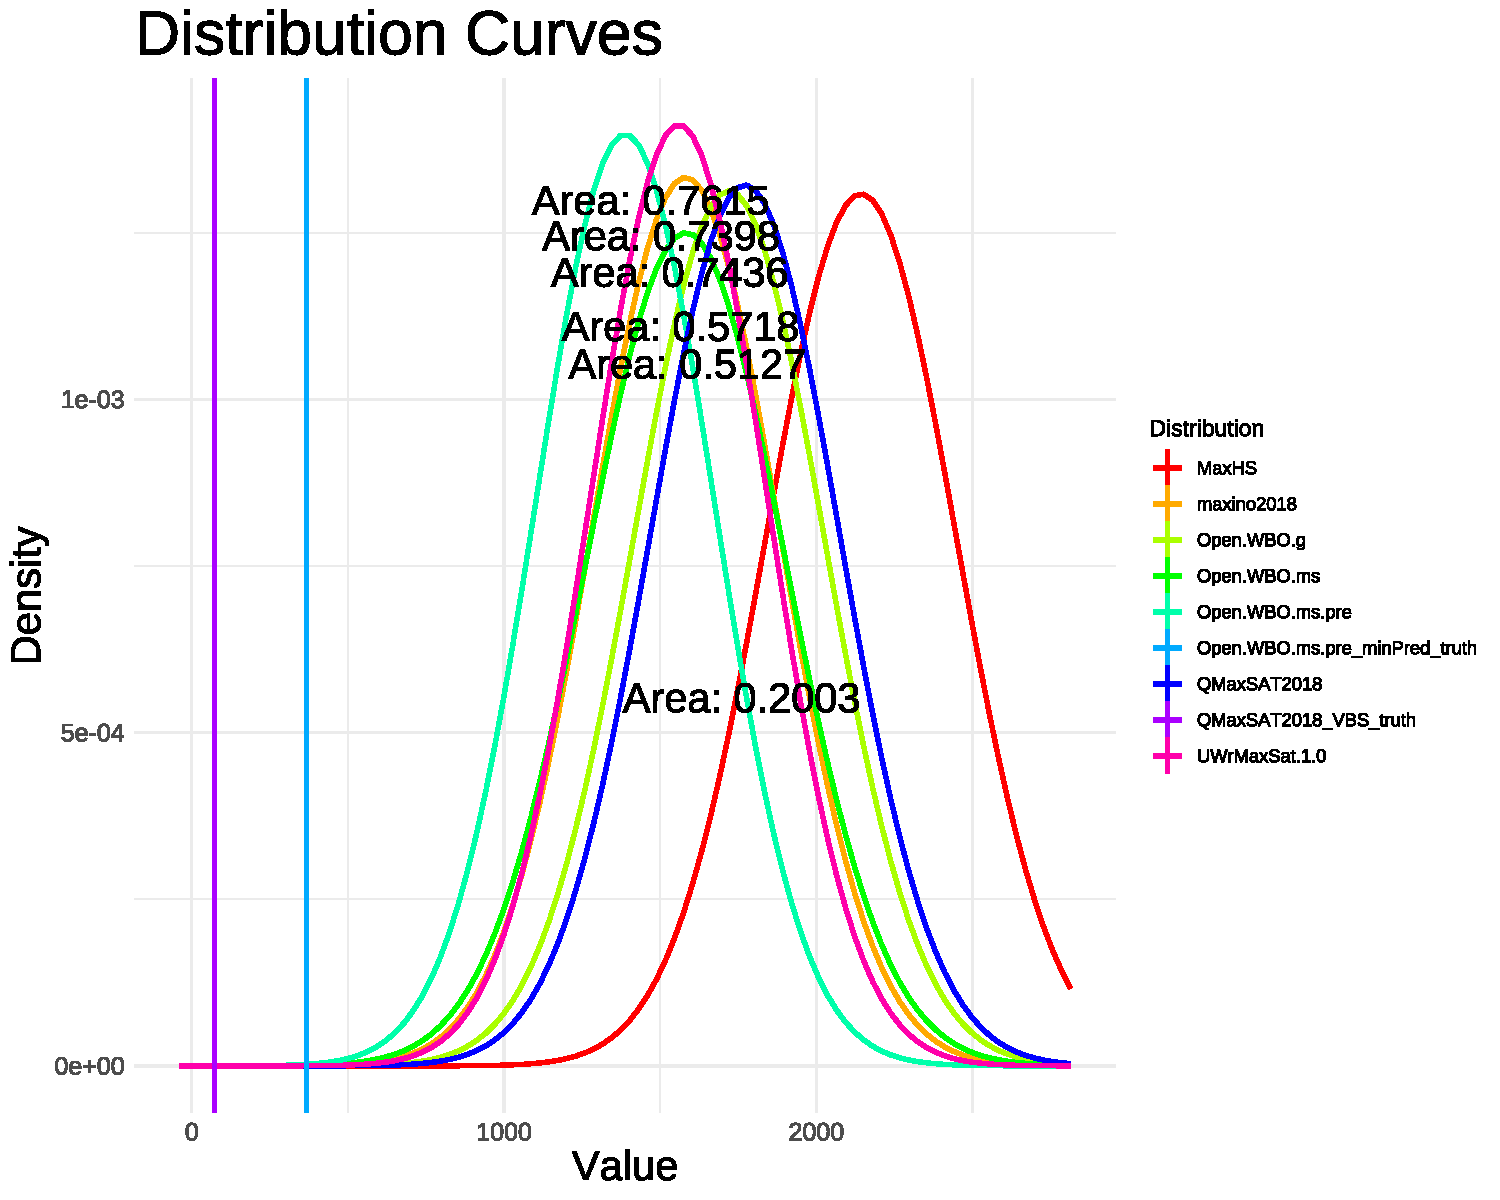
\includegraphics[width=.49\textwidth]{plots/Appendix/1bpi_2knt_gwcnft.wcnf.pdf}
    \caption[Sub-portfolio Selection: Examples from MAXSAT19-UCMS]{Sub-portfolio selection for two example instances from MAXSAT19-UCMS based on the optimal $p_{\cap}$ values}
    \label{fig:appendix_maxsat}
\end{figure}

% \begin{figure}[t]
% \centering
%     \centerline{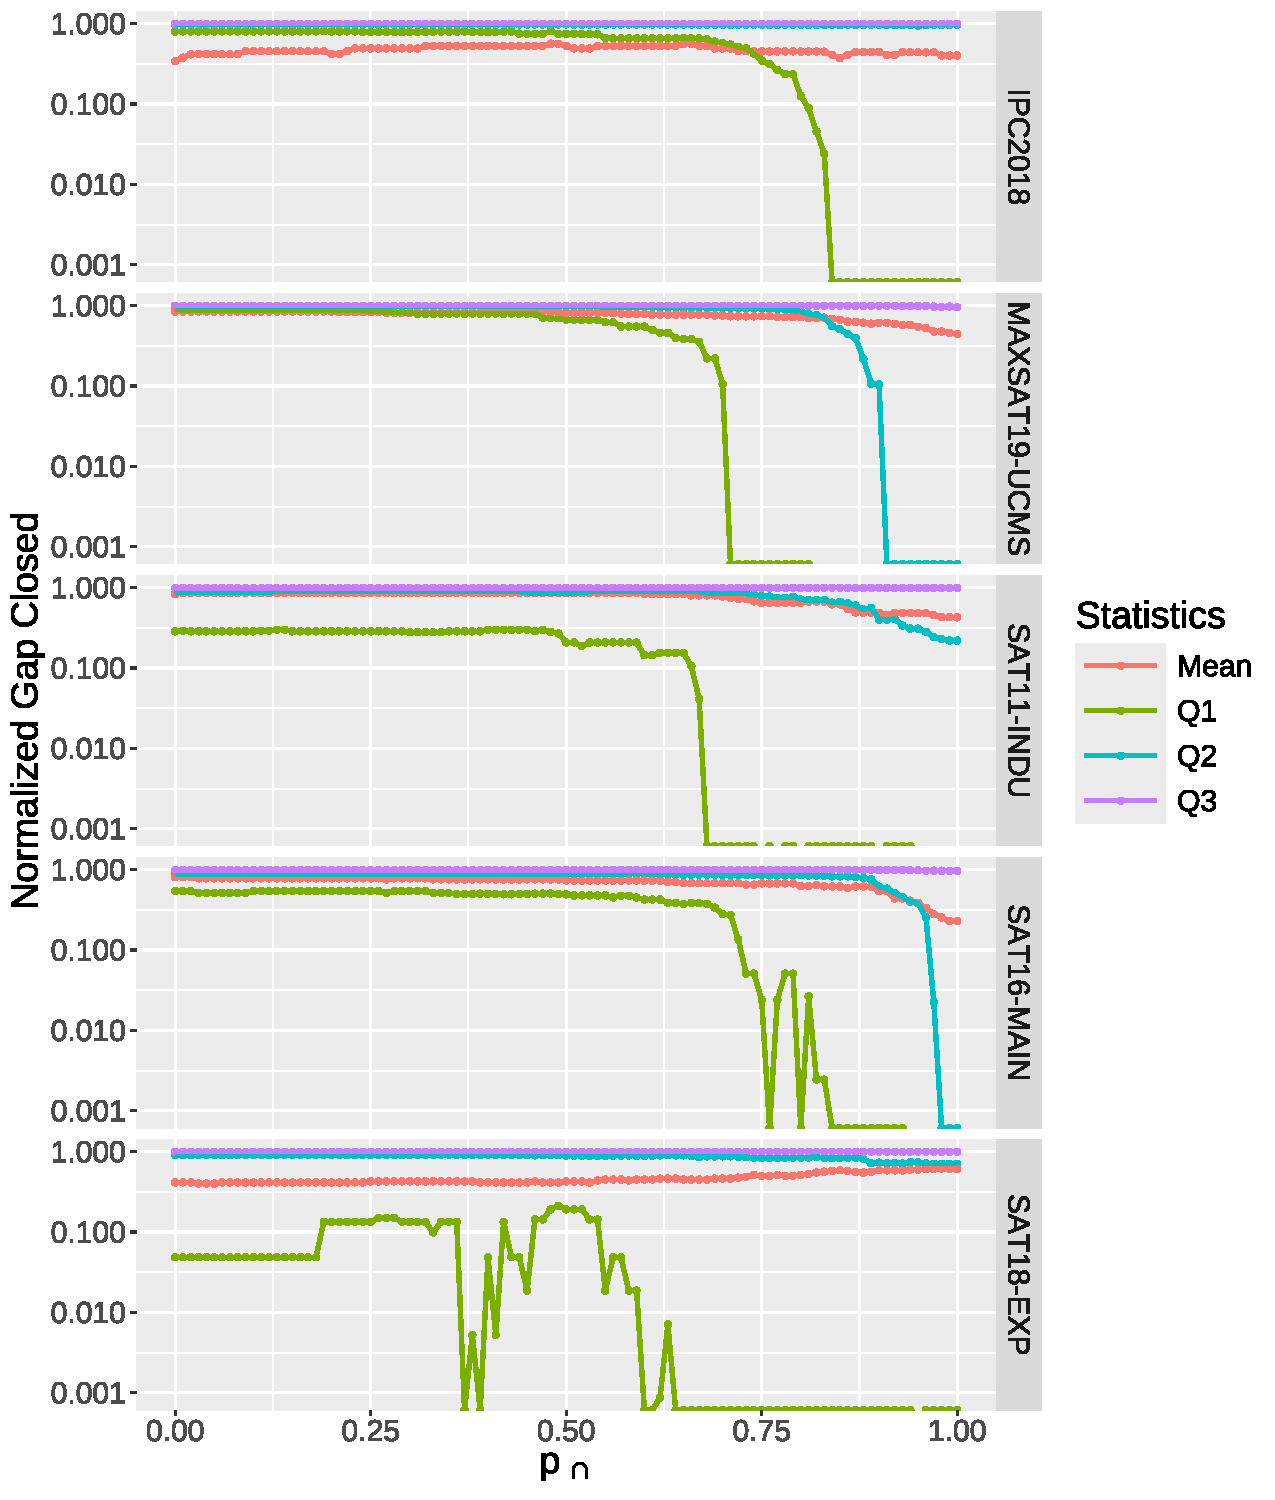
\includegraphics[width=\linewidth]{plots/pcap_rj_sensitivity_x_theta_y_runtime_facet.pdf}}
%     \caption{Sensitivity of portfolio performance to $p_{\cap}$. This plot refers to RJ model - Regression Ranger model with Jackknife uncertainty estimation method. The plot illustrates the mean, Q1 (25th percentile), Q2 (50th percentile), and Q3 (75th percentile) runtime performance of each scenario for various values of $p_{\cap}$ as defined in Equation~\ref{eq:7}. Note the log scale for the normalized gap closed.}
%     \label{fig:sensitivity_pcap_ri}
% \end{figure}